% !TeX root = RJwrapper.tex
\title{An Algorithm For Spatial Mapping Using a Hexagon Tilegram, With
Application to Australian Maps}
\author{by Stephanie Kobakian, Dianne Cook}

\maketitle

\abstract{%
This algorithm creates a hexagon to represent each of the spatial
polygons provided. It allocates these hexagon in a manner that preserves
the spatial relationship of the areas. It showcases spatial
distributions, by emphasising the small geographical regions that are
often difficult to locate on large geographic maps.
}

% Any extra LaTeX you need in the preamble

\hypertarget{introduction}{%
\subsection{Introduction}\label{introduction}}

Spatial distributions have utilised alternative representations of
geography for many years. In modern times interactivity and animation
have begun to play a larger role, as alternative representations have
been popularised by online news sites, with a focus on public
consumption. Applications are increasingly widespread, especially in the
areas of disease mapping, and election results.

\hypertarget{motivation}{%
\subsection{Motivation}\label{motivation}}

Spatial distributions of people and human related statistics can be
misrepresented in geographic maps. Populations congregate around major
cities and vertical living is increasingly common. Population statistics
often requires dividing people into smaller, measurable areas.
Government bodies such as the Australian Bureau of Statistics, or
intentionally segregated organisations, like the Australian Electoral
Commission hold the responsibility of the division. Australia is an
example of strong urbanisation, the rural areas are often sparsely
populated in comparison to the urban centres. To divide the population
equally, the square meters of the geographic areas differ dramatically
in size.

Alternative mapping methods allow increased understanding of the spatial
distribution of a variable across the population. Alternative maps allow
the focus to be placed on the distribution of the statistics between the
groups of areas.

Extremely small geographic areas are lost on large geographic maps,
small inner areas of Sydney or Melbourne are not easily compared at a
high level. Cartograms place importance on the statistic of interest,
allowing distorted map space on the display to represent differences in
the statistic. These maps rely on the statistic of interest to determine
the layout, and for Australia, often fail to preserve a recognisable
view. Tilegrams allow preservation of spatial relationships as they
decrease the emphasis on the amount of geographic area considered to be
interesting. These maps focus on the relationship between neighbours, in
considering aggregated statistics of heterogeneous regions.

Our case is an extension of these concepts. Extending the tilegram to
Australian applications required preserving the spatial relationships.
It emphasises the capital cities as population hubs, and recognises the
populations distributed across the large rural areas.

\hypertarget{algorithm}{%
\section{Algorithm}\label{algorithm}}

Our solution operates on a set of polygons. There are parameters used in
the process that may be provided, or will be automatically derived. All
necessary functions are exported, with a main function
\texttt{create\_hexmap} used to step through these automatically.

\hypertarget{parameters}{%
\subsection{Parameters}\label{parameters}}

The \texttt{create\_hexmap} function requires several parameters, if
they are not provided, the information will be derived from the polygon
set used.

\textbf{The following must be provided to \texttt{create\_hexmap}:}

\begin{Schunk}

\begin{tabular}{l|l}
\hline
parameter & description\\
\hline
shp & an Rdata object containing the polygon information\\
\hline
shp\_path & character string location of the shape file that contains the polygon information\\
\hline
sf\_id & name of a unique column that distinguishes areas\\
\hline
capital\_cities & a data frame of reference locations used to allocate hexagons\\
\hline
\end{tabular}

\end{Schunk}

The polygon set of Local Government Areas in Tasmania in 2016 is stored
in the sugarbag package data as \texttt{tas\_lga}. A single column of
the data set must be used as a unique identifier of areas. In this case,
the unique LGA codes associated with each LGA have been used, their
names could have also been used.

The centre of the population hubs are used to distribute areas around
the closest capital city.

\textbf{The following parameters will be determined within
\texttt{create\_hexmap} if not provided. They are created throughout the
following example:}

\begin{Schunk}

\begin{tabular}{l|l}
\hline
parameter & description\\
\hline
buffer\_dist & a float value for distance in degrees to extend beyond the - geometry provided\\
\hline
hex\_size & a float value in degrees for the diameter of the hexagons\\
\hline
hex\_filter & amount of hexagons around centroid to consider for allocation\\
\hline
width & the angle used to filter the grid points around a centroid\\
\hline
\end{tabular}

\end{Schunk}

When utilising individual \texttt{sugarbag} functions, we recommend the
following approach:

\hypertarget{polygon-information}{%
\subsection{Polygon Information}\label{polygon-information}}

Begin with a set of polygons. The set should be provided as an
\texttt{sf} object, this is a data frame containing a \texttt{geometry}
column. The \texttt{read\_shape} function can assist in creating this
object. We will use the Local Government Areas of Tasmania, sourced from
the Australian Bureau of Statistics.

\begin{Schunk}
\begin{figure}
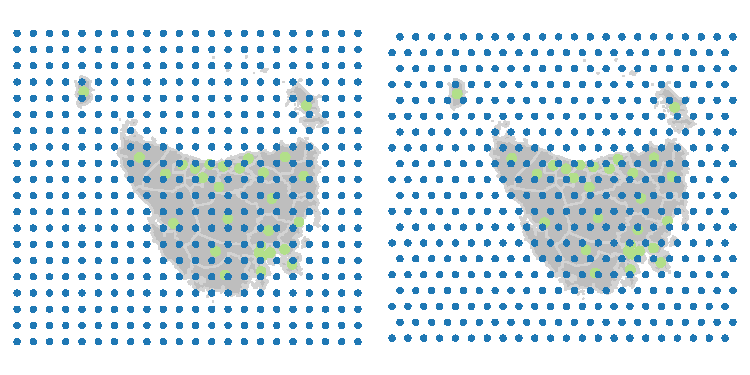
\includegraphics{algorithmRjournal_files/figure-latex/unnamed-chunk-3-1} \caption[lga Local Government Areas and derived centroids]{lga Local Government Areas and derived centroids.}\label{fig:unnamed-chunk-3}
\end{figure}
\end{Schunk}

\hypertarget{hexagon-grid}{%
\subsection{Hexagon grid}\label{hexagon-grid}}

Each new hexagon will need to tessellate, a grid is created to ensure a
close point is found, that will allow all areas to tessellate, this is
inspired by tilegrams. The grid of possible hexagon centroids can be
made using the \texttt{create\_grid} function. The grid creation takes
several steps. It requires the centroids, the hexagon size and the
buffer distance.

\hypertarget{step-1-expand-the-grid}{%
\subsubsection{Step 1: Expand the grid}\label{step-1-expand-the-grid}}

One sequence is created for longitude columns, and another for latitude
rows.

The sequences begin at the minimum longitude or latitude, minus the
buffer distance. Equally spaced intervals the size of the hexagons are
created up to the maximum longitude or latitude, plus the buffer
distance.

An individual point is created from all intersections of the longitude
columns and latitude row sequences.

\begin{Schunk}

\includegraphics{algorithmRjournal_files/figure-latex/plot_grid-1} \end{Schunk}

A square grid will not facilitate tessellated hexagons. Every second
latitude row of points will be shifted right by half of the hexagon
size.

\begin{Schunk}

\includegraphics{algorithmRjournal_files/figure-latex/plot_shift-1} \end{Schunk}

Each point is now given an ID.

\hypertarget{step-2-rolling-windows}{%
\subsubsection{Step 2: Rolling windows}\label{step-2-rolling-windows}}

Not all of the grid points will be used, especially if islands impact
the overall space covered. To filter the grid for appropriate points for
allocation, the \texttt{create\_buffer} function is called from
\texttt{create\_grid}. It finds the amount of columns and rows needed to
best capture the set of centroids.

The rows and columns are divided into 20 groups. The amount of rows in
each latitude group and the amount of columns in each longitude group
are then used as the width of manual rolling windows. This will tailor
the available points to the areas most likely to be used. It helps
reduce amount of time taken.

The specific rows and columns in the rolling windows are defined.The
first rolling window function finds the minimum and maximum centroid
values for the sliding groups of longitude columns and the groups of
latitude rows.

The second rolling window function finds the average of the rolling
minimum and rolling maximum centroid values, for the longitude columns
and latitude rows.

\hypertarget{step-3-filtering-the-grid}{%
\subsubsection{Step 3: Filtering the
grid}\label{step-3-filtering-the-grid}}

Only the grid points between the rolling average of the minimum and
maximum centroid values are kept, for each row and column of the grid.

\begin{Schunk}

\includegraphics{algorithmRjournal_files/figure-latex/plot_buffer-1} \end{Schunk}

\hypertarget{centroid-to-focal-point-distance}{%
\subsection{Centroid to focal point
distance}\label{centroid-to-focal-point-distance}}

For each polygon centroid in the set, the distance to each of the focal
points provided is recorded. The closest focal point name, the distance
to the polygon centroid, and the angle from focal point to polygon
centroid will be added to the polygon's row, in the polygon data set. To
minimise time taken for this step, only Tasmania's capital city Hobart
has been provided.

The distance between the polygon centroid and it's closest focal point
data set is used to order the data set for allocation. The points are
arranged in ascending order, from the centroid closest to any of the
focal points, to the furthest.

\hypertarget{allocation-of-centroids}{%
\subsection{Allocation of centroids}\label{allocation-of-centroids}}

The distance around a centroid to consider for possible hexagon
locations is determined by the hex\_filter. It multiplies the amount
given by hex\_filter, by the size of the hexagons to find the distance.

Allocation of all centroids can now take place using the set of polygon
centroids and the hexagon map grid. For each polygon centroid, only the
hexagon grid points that have not yet been used can be considered.
Allocate each centroid, beginning with the closest centroid to a focal
point. This will preserve spatial relationship with the capital, as the
inner areas will be allowed closest to the capital, and the areas that
are further will be accommodated after.

The filter parameter is used to subset possible grid points to only
those surrounding the polygon centroid within the filter distance,
smaller distance will increase speed, but can decrease accuracy.

The following example considers one of the Local Government Areas. These
steps are repeated for each polygon.

\hypertarget{step-1-filter-the-grid-for-unassigned-hexagon-points}{%
\subsubsection{Step 1: Filter the grid for unassigned hexagon
points}\label{step-1-filter-the-grid-for-unassigned-hexagon-points}}

Keep only the available hexagon points, this will prevent multiple areas
being allocated to the same hexagon.

\hypertarget{step-2-filter-the-grid-points-for-those-closest-to-the-centroid}{%
\subsubsection{Step 2: Filter the grid points for those closest to the
centroid}\label{step-2-filter-the-grid-points-for-those-closest-to-the-centroid}}

This will allow only the closest points, that are not assigned, to be
considered.

Create a box of possible hexagon locations around the centroid. The
bottom of the box will not be square as the buffer has already removed
unnecessary points from over the ocean.

\begin{Schunk}

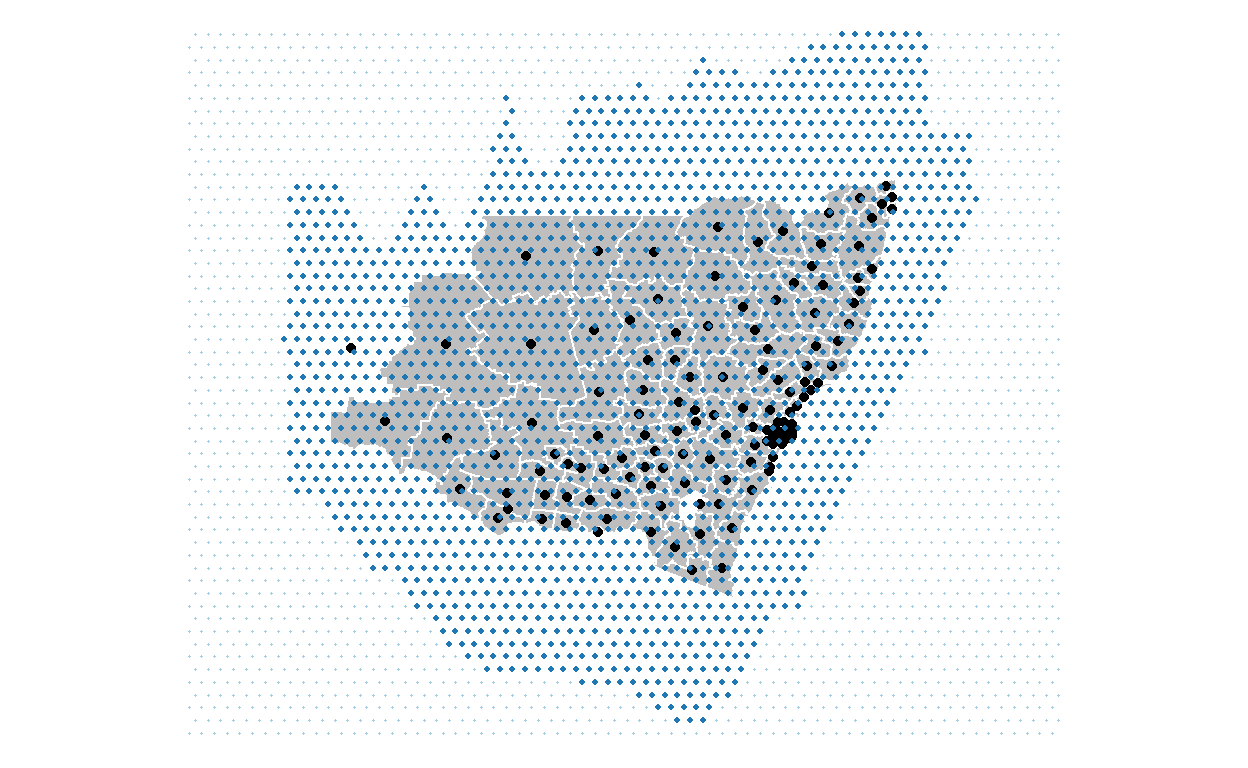
\includegraphics{algorithmRjournal_files/figure-latex/unnamed-chunk-12-1} \end{Schunk}

The algorithm removes the outer corners of the square, creating a circle
of points, by only keeping points within a certain radius around the
original centroid location.

\begin{Schunk}

\includegraphics{algorithmRjournal_files/figure-latex/unnamed-chunk-14-1} \end{Schunk}

The width parameter is now used. Of the remaining points, a slice is
taken. This uses the angle from the closest capital city, to the current
centroid. If it is not the closest to the capital there may have been
points available that were taken by closer centroids. This allows the
spatial relationship to be preserved, even when it gets allocated to a
hexagon that is further from the city centre. This angle begins at 30
degrees by default, and may increase if necessary.

If no available hexagon grid point is found within the original filter
distance and angle, the distance is expanded, only when a maximum
distance is reached will the angle expand to accommodate more possible
grid points.

The allocation is returned and combined with the data relating to each
polygon.

\begin{Schunk}

\includegraphics{algorithmRjournal_files/figure-latex/unnamed-chunk-16-1} \end{Schunk}

This area was the very closest to the Hobart central point ( coloured
pink) provided in the capital cities data set, it gets a hexagon point
(coloured blue) extremely close to it's centroid (coloured green).

\begin{Schunk}

\includegraphics{algorithmRjournal_files/figure-latex/unnamed-chunk-19-1} \end{Schunk}

The following code creates a map for all the Local Government Areas in
Tasmania:

\begin{Schunk}
\begin{Sinput}
# Create centroids set
centroids <- create_centroids(tas_lga, "LGA_CODE16")
# Create hexagon location grid
grid <- create_grid(centroids = centroids,
    hex_size = 0.25,
    buffer_dist = 1.2)
# Allocate polygon centroids to hexagon grid points
hex_allocated <- allocate(
  centroids = centroids,
  hex_grid = grid,
  sf_id = "LGA_CODE16",
  # same column used in create_centroids
  hex_size = 0.25,
  # same size used in create_grid
  hex_filter = 10,
  focal_points = capital_cities %>% filter(points == "Hobart"),
  width = 30,
  verbose = FALSE
)
\end{Sinput}
\end{Schunk}

\begin{Schunk}

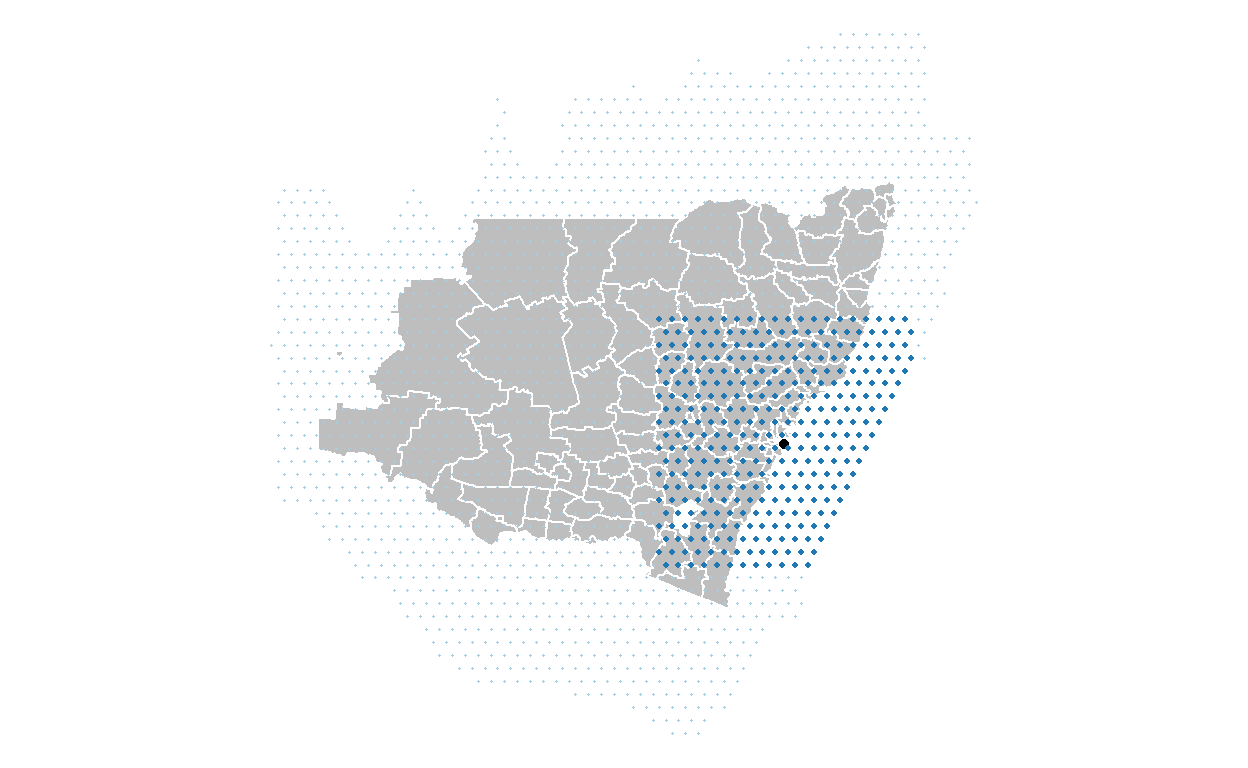
\includegraphics{algorithmRjournal_files/figure-latex/unnamed-chunk-20-1} \end{Schunk}

\hypertarget{summary}{%
\subsection{Summary}\label{summary}}

It is possible to use alternative maps to communicate spatial
distributions. Current methods do not always work for Australia due to
the large gaps between densely populated capital cities.

\hypertarget{code}{%
\subsection{Code}\label{code}}

This map algorithm is found in the \texttt{sugarbag} package, currently
available on github: \url{https://github.com/srkobakian/sugarbag}

\bibliography{algorithmbib}


\address{%
Stephanie Kobakian\\
Queensland Univeristy of Technology\\
\\
}
\href{mailto:stephanie.kobakian@monash.edu}{\nolinkurl{stephanie.kobakian@monash.edu}}

\address{%
Dianne Cook\\
Monash University\\
\\
}
\href{mailto:dicook@monash.edu}{\nolinkurl{dicook@monash.edu}}

